\documentclass[12pt]{article}

\usepackage[utf8]{inputenc}
\usepackage{indentfirst}
\usepackage{float}
\usepackage{amsmath}
\usepackage{makecell}
\usepackage{xurl}

\usepackage{sbc-template}

\usepackage{graphicx,url}

\usepackage[brazil]{babel}
%\usepackage[latin1]{inputenc}

\def\UrlBreaks{\do\/\do-\do\_\do\.\do\~}

\graphicspath{ {../tcc/images/} }

\sloppy

\title{Dinâmica para identificação e análise de riscos em equipes ágeis}

\author{Amanda Martins Oliveira\inst{1}, Jean Carlo Rossa Hauck\inst{1}}

\address{
  Departamento de Informática e Estatística -- Universidade Federal de Santa Catarina 
  (UFSC)\\
  Florianópolis -- SC -- Brasil
  \email{amanda.martins.oliveira@grad.ufsc.br, jean.hauck@ufsc.br}
}

\begin{document}

\maketitle
\begin{abstract}
  The increasing adoption of agile methods brings flexibility but also challenges in risk management, often overlooked. This work proposed and evaluated a playful dynamic to assist this process in agile teams.
  Based on a theoretical review of agile risk management and gamification, the dynamic was developed and applied in software development teams and in classrooms. Results showed that the proposal was well-received, contributing to engagement and facilitating the collaborative identification and discussion of risks.
\end{abstract}

\begin{resumo}
  A crescente adoção de métodos ágeis traz flexibilidade, mas também desafios na gestão de riscos, muitas vezes negligenciada. Este trabalho propôs e avaliou uma dinâmica lúdica para auxiliar esse processo em equipes ágeis.
  Baseada em revisão teórica sobre gestão de riscos ágil e gamificação, a dinâmica foi desenvolvida e aplicada em equipes de desenvolvimento de software e em sala de aula. Os resultados demonstraram que a proposta foi bem recebida, contribuindo para o engajamento e facilitando a identificação e discussão colaborativa de riscos.
\end{resumo}

\section{Introdução}
A crescente adoção de metodologias ágeis no desenvolvimento de \textit{software} e gestão de projetos \cite{AgileManifest, AgileGuide}, como Scrum e Kanban, destaca sua flexibilidade e adaptabilidade. Contudo, a gestão de riscos, embora essencial para o sucesso dos projetos, frequentemente não é estruturada em contextos ágeis, tornando equipes vulneráveis a imprevistos que afetam prazos, custos e qualidade do produto \cite{Afshari, Zahedi}.

Este trabalho aborda essa lacuna, propondo uma dinâmica lúdica e acessível para a gestão de riscos em equipes ágeis, com a hipótese de que tal ferramenta apoie a identificação e análise de riscos para entregas mais consistentes e resilientes. A pesquisa se justifica pela falta de práticas explícitas de gestão de riscos em métodos ágeis \cite{LopesSamueldeSouza2022ARMF}, onde modelos tradicionais se mostram inflexíveis por exigirem documentação extensa ou processos pesados. A dinâmica gamificada alinha-se a abordagens recentes que utilizam jogos sérios para promover engajamento e aprendizado na gestão de projetos de software, tornando a identificação de riscos mais colaborativa e intuitiva.

O objetivo é contribuir com uma ferramenta prática, replicável e de baixo custo que pode ser adotada por diferentes equipes e organizações, esperando incentivar a adoção de gestão de riscos mais sistemática e acessível no desenvolvimento ágil de \textit{software}.

\section{Metodologia de pesquisa} 

Este estudo adotou uma metodologia em quatro etapas principais:

\begin{enumerate}
\item \textbf{Fundamentação teórica}: Nesta etapa, foram revisados conceitos fundamentais da literatura relacionados a gerência de projetos, métodos ágeis e gestão de riscos. Isso incluiu a fundamentação dos principais conceitos sobre gerência de projeto, gestão de riscos, métodos ágeis e gamificação.
\item \textbf{Análise do estado da arte}: Consistiu em uma revisão sistemática da literatura (MSL) para o levantamento de estudos correlacionados com o tema, feita como continuidade do mapeamento feito por \cite{garcia2023agreed}, seguindo os procedimentos definidos por \cite{PETERSEN20151} e \cite{Petersen}. As atividades desta etapa incluíram a definição do protocolo de pesquisa, seleção dos estudos e análise dos resultados.
\item \textbf{Desenvolvimento da dinâmica}: A partir das etapas anteriores, foi criada a dinâmica para identificação e análise de riscos em equipes ágeis. Esta etapa é composta pelas atividades de identificação de objetivos, análise dos usuários, desenvolvimento da proposta de solução, definição do escopo da gamificação e estudo de viabilidade, análise e design e desenvolvimento da gamificação.
\item \textbf{Avaliação da dinâmica e aplicação do estudo de caso}: Nesta etapa final, a dinâmica desenvolvida foi aplicada, executando um estudo de caso e realizando a avaliação e validação da mesma. As atividades incluíram o planejamento do estudo de caso, a realização do estudo de caso e a análise dos resultados do estudo de caso.
\end{enumerate}

A questão geral de pesquisa foi definida como: “Como as organizações de \textit{software} integram práticas explícitas de gerenciamento de riscos em métodos ágeis?”, e foi desdobrada em quatro questões de análise detalhada: 1) Qual contexto de uso de práticas de gestão de riscos nos métodos ágeis?; 2) Quais práticas de gestão de riscos são introduzidas nos métodos ágeis?; 3) Quais tipos de riscos são gerenciados?; 4) Quais os resultados da introdução de práticas explícitas de gestão de riscos nos métodos ágeis?. O escopo da pergunta de pesquisa seguiu a estrutura PICOC (População, Intervenção, Comparação, Resultados e Contexto).

A string de busca utilizada nas bibliotecas digitais IEEEXplore, ACM Digital Library e Scopus foi: \textit{“risk” AND (“agile” OR “scrum” OR “xp” OR “extreme programming” OR “lean” OR “kanban” OR “scrumban” OR “fdd” OR “feature driven development” OR “crystal” OR “iterative development”) AND “software”}. Os critérios de inclusão focaram em estudos primários revisados por pares, em inglês, com no mínimo 4 páginas e publicados a partir de 2021. Os critérios de exclusão visaram eliminar trabalhos teóricos não aplicados empiricamente, duplicados, com texto completo indisponível ou não focados em desenvolvimento de software. O processo de seleção resultou em 7 estudos primários após três ciclos de filtragem.

Os estudos selecionados foram predominantemente conduzidos na indústria (71\%), com 50\% deles utilizando estudos de caso. Em termos de métodos ágeis, o \textit{Scrum} foi mencionado em 2 estudos, XP, DAD e SAFe em 1 estudo cada, embora 4 estudos não tenham especificado um método ágil. Observou-se que 57\% dos estudos foram aplicados em apenas 1 organização. As práticas de gestão de riscos introduzidas nos métodos ágeis se dividiram em duas estratégias: usar práticas ágeis existentes ou introduzir novas práticas adaptadas. Todos os 7 estudos selecionados relataram impactos positivos da introdução de práticas explícitas de gerenciamento de riscos, e 43\% destacaram que isso ocorreu sem comprometer a agilidade dos métodos ágeis. Exemplos incluem a melhoria na eficiência, qualidade das entregas e maior conhecimento sobre gestão de riscos. Os estudos primários selecionados identificaram um total de 97 riscos, agrupados por meio da taxonomia de \cite{carr_1993}. O atributo com maior frequência de riscos foi “Schedule”, da classe “Program Constraints”, identificado em 4 dos estudos primários.

\section{Tarot dos riscos}
Nesta seção é apresentada o Tarot dos riscos, dinâmica ideada para apoiar o processo de identificação e análise de riscos em equipes ágeis.

\subsection{Público alvo e contexto}

A dinâmica foi projetada para equipes ágeis atuando em desenvolvimento de software, onde a gestão de riscos é frequentemente implícita, sem etapas estruturadas ou práticas específicas para a identificação e análise de riscos.

A análise de participantes com base em dados demográficos do setor brasileiro indica que a maioria dos profissionais do setor de TI no Brasil tem menos de 30 anos \cite{jetbrains2023dev}, com uma média de 33 anos em Santa Catarina \cite{acate}. O setor é predominantemente masculino, e mais de 85\% dos profissionais possuem graduação em áreas de tecnologia \cite{revelo2021tecnologia}. Especialidades como Full-stack, Back-end e Front-end são as mais representativas. Além disso, 63\% dos profissionais preferem o uso do Scrum em nível de equipe \cite{17_agile_report}, o que reforça a relevância de soluções gamificadas para esse público adaptado a metodologias ágeis.

\subsection{Objetivos}
Os principais objetivos da dinâmica incluem: facilitar a identificação de riscos de forma interativa e acessível para que equipes detectem riscos potenciais em projetos de software. A intenção é oferecer um espaço estruturado e colaborativo para que os membros da equipe reconheçam riscos potenciais e alinhem ações de mitigação, promovendo maior clareza e previsibilidade no trabalho, sem comprometer a agilidade dos processos.

Além disso, a dinâmica visa promover a análise colaborativa entre os membros da equipe, estimulando a discussão e o alinhamento sobre a aplicabilidade, probabilidade e impacto dos riscos. Outro objetivo é guiar a equipe na seleção dos riscos mais críticos que exigem atenção imediata e planejamento de respostas. A proposta busca também engajar os participantes, transformando a tarefa de gestão de riscos, que pode ser percebida como árida, em uma atividade lúdica e motivadora. Por fim, a dinâmica serve como ferramenta pedagógica para equipes e estudantes que buscam compreender melhor os conceitos e a prática da gestão de riscos em um contexto ágil.

\subsection{Definição dos recursos de gamificação}
Os elementos de gamificação da dinâmica foram definidos para facilitar a identificação e análise de riscos de forma interativa e engajadora. O componente central são as Cartas de Risco, totalizando 32 unidades. Esse número foi determinado com base na taxonomia de riscos de \cite{carr_1993}, priorizando os riscos mais citados no Mapeamento Sistemático da Literatura (MSL) de \cite{garcia2023agreed} e na continuidade deste estudo, cobrindo 84,4\% dos riscos identificados. Visualmente, as cartas apresentam ilustrações únicas no estilo “Pokémon”, geradas com auxílio de inteligência artificial (utilizando Pixlr Image Generator), e cada uma contém um nome lúdico, o nome técnico do risco, a classe do risco, uma pergunta principal e perguntas auxiliares para aprofundar a análise. A anotamia da carta pode ser observada na figura abaixo.

\begin{figure}[H]
  \centering
  \caption{\label{anatomia-carta-completa} Anatomia da carta}
  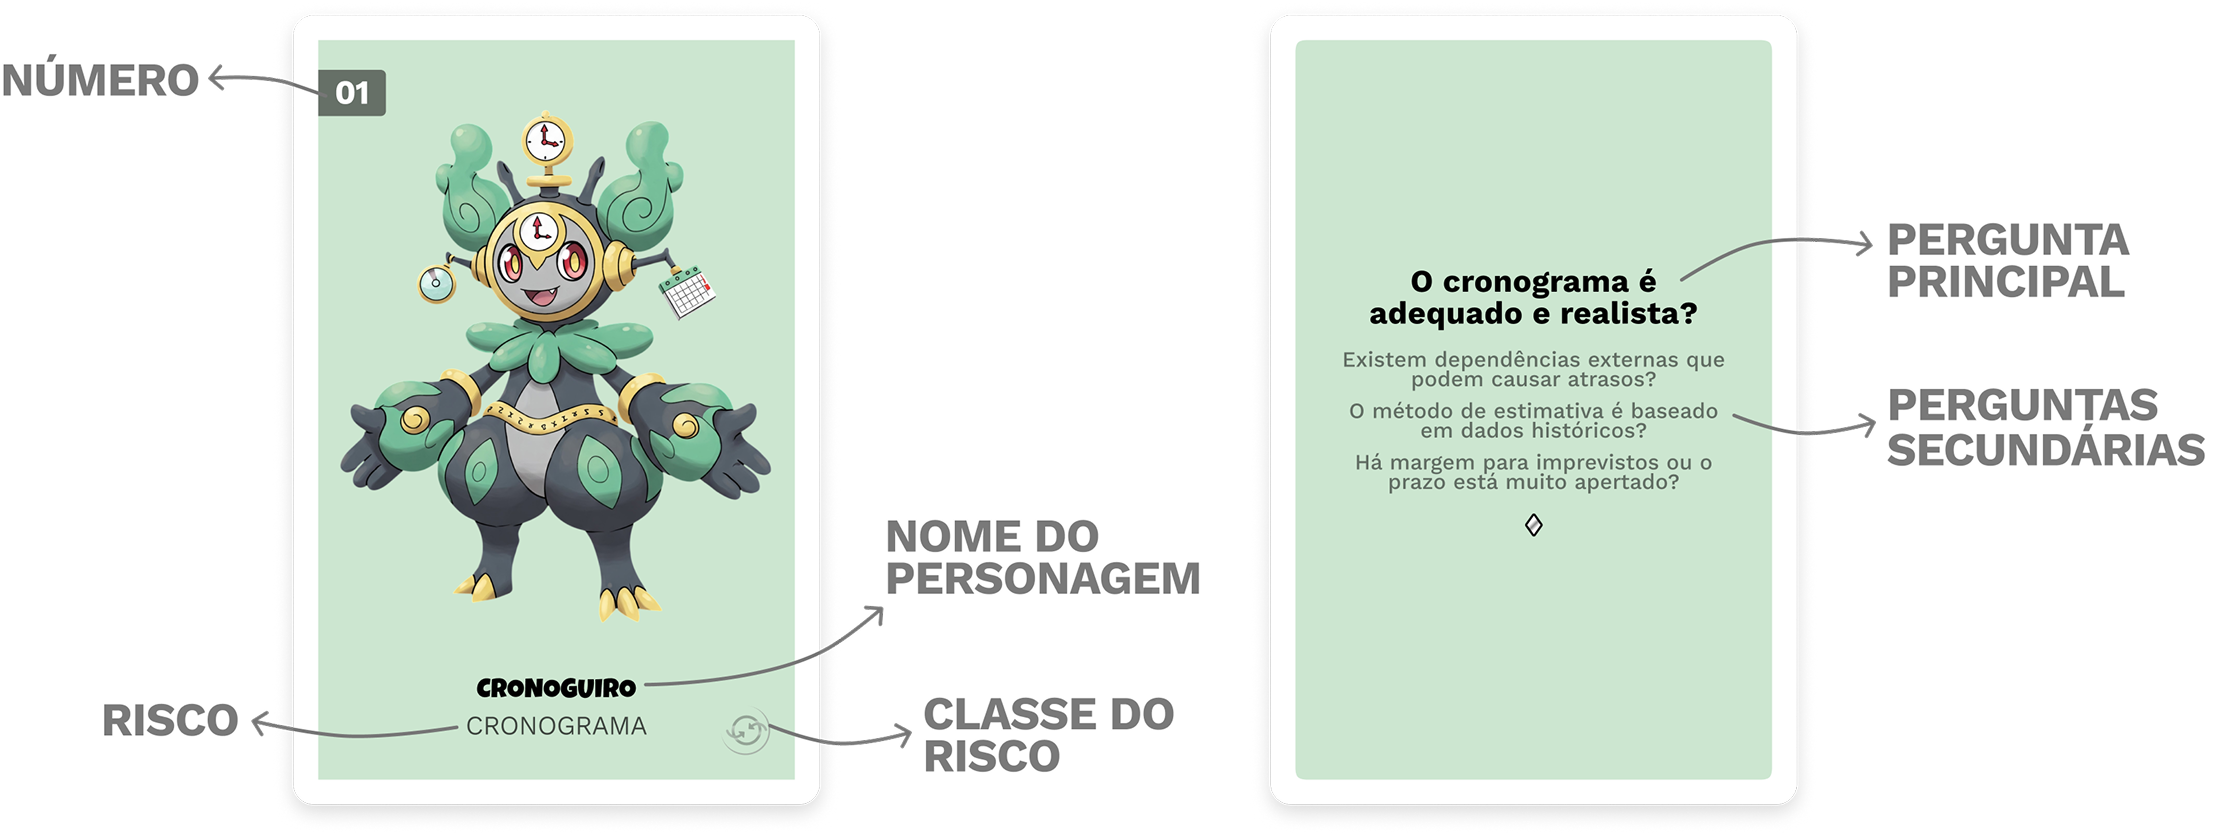
\includegraphics[width=0.85\textwidth]{anatomia-carta-completa}
\end{figure}

Além das cartas, a dinâmica utiliza:

\begin{itemize}
  \item \textbf{Moedas para votação}: feitas para a priorização dos riscos durante a segunda etapa da dinâmica, mas também como método para incentivar a participação ativa na primeira etapa.
  \item \textbf{Manual de regras}: meio de consulta às regras e recomendações da dinâmica, fornecido para guiar a condução.
  \item \textbf{Post-its e canetas}: materiais auxiliares que permitem aos participantes escreverem riscos específicos relacionados a cada carta, fomentando a individualização e o detalhamento.
\end{itemize}

\begin{figure}[H]
  \centering
	\caption{\label{tarot-fisico} Materiais que compõem a dinâmica}
  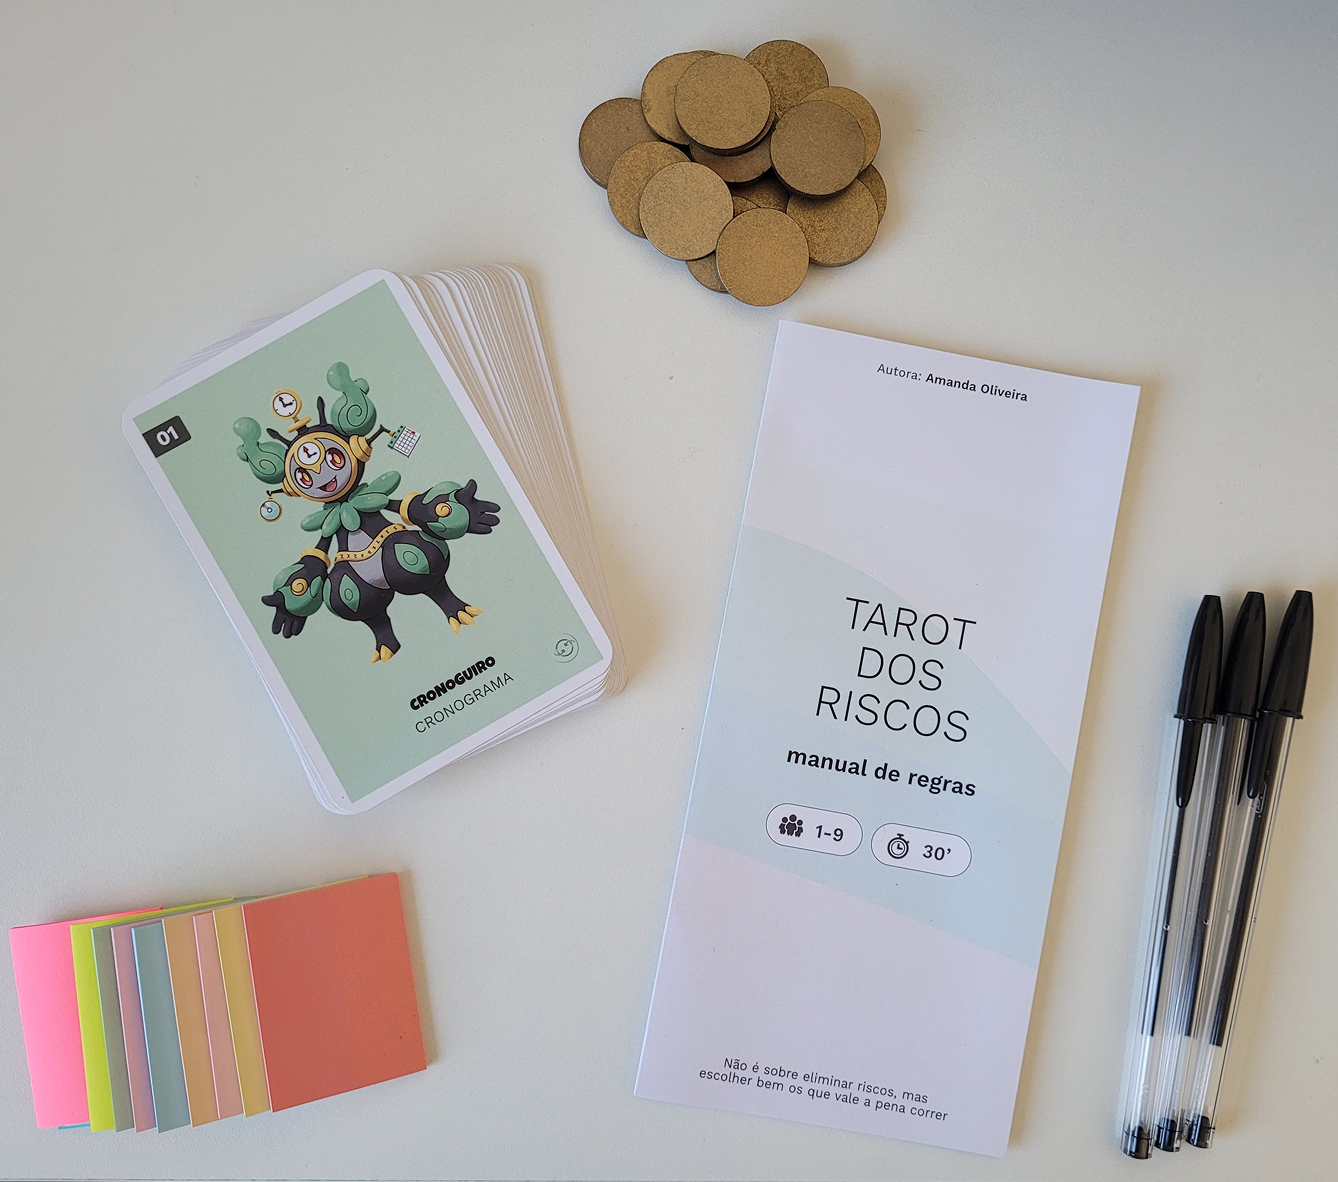
\includegraphics[width=0.55\textwidth]{tarot-fisico}
\end{figure}

A estética geral do jogo busca ser leve, convidativa e divertida, desmistificando a gestão de riscos e tornando-a mais acessível. As cartas, elementos visuais, e a temática sugerida pelo nome “Tarot dos Riscos” contribuem para uma experiência que evoca a ideia de “prever o futuro” e antecipar desafios de forma proativa.

\section{Avaliação da dinâmica}
\subsection{Definição da avaliação}

A avaliação da dinâmica buscou verificar se os objetivos propostos foram alcançados, além de analisar a experiência dos participantes quanto ao engajamento, clareza e aplicabilidade prática da atividade. Para isso, foi elaborado um questionário com base no modelo MEEGA+ \cite{MEEGA}, contendo afirmativas em escala de concordância, além de campos abertos para observações qualitativas. O instrumento avaliativo foi desenhado para capturar a percepção dos participantes de forma ampla, permitindo uma análise quantitativa e qualitativa da experiência.

\subsection{Estratégia de aplicação}

A mecânica do jogo foi projetada para guiar as interações e o fluxo da dinâmica, desde a apresentação dos riscos até sua priorização colaborativa. O design buscou criar um processo flexível que promovesse o pensamento crítico e a colaboração. Para isso, a dinâmica é estruturada em duas fases principais:

\begin{enumerate}
\item \textbf{Identificação e mapeamento dos riscos}: Esta etapa inicial foca na associação entre os riscos genéricos, apresentados nas cartas, e os riscos reais e específicos enfrentados pela equipe. O facilitador lê uma carta e a equipe avalia coletivamente sua aplicabilidade ao projeto; se pertinente, a carta é mantida. Para cada carta aplicável, os participantes escrevem individualmente em post-its os riscos práticos e específicos relacionados, que são agrupados ao redor da carta. Um momento de discussão e alinhamento é aberto, focando na análise sem desviar para soluções.
\item \textbf{Votação e priorização dos riscos}: Após o mapeamento, a equipe avança para a priorização, que utiliza uma mecânica inspirada na técnica “Buy a Feature”. Cada participante recebe uma quantidade inicial de 3 moedas, com moedas adicionais concedidas a cada 5 post-its escritos na etapa anterior, incentivando a contribuição. Com as moedas, cada um as distribui entre as cartas que considera mais críticas, forçando uma priorização cuidadosa. Após a votação, os riscos são classificados pela quantidade de moedas acumuladas e priorizados com base neste ordenação.
\end{enumerate}

O facilitador é fundamental para garantir a condução eficaz da dinâmica, sendo responsável pela preparação, condução das etapas, mediação das discussões e gestão do tempo. A equipe também pode optar pela auto-organização, revezando-se nas funções do facilitador. A preparação envolve a escolha do deck de cartas (completo, básico ou temáticos), a organização dos materiais e a familiarização com o manual de regras.

\subsection{Aplicação e coleta de dados}
A dinâmica foi aplicada com dois grupos distintos: estudantes universitários e profissionais do Laboratório Bridge. A aplicação com estudantes acontece de forma presencial  em sessões de em média 30 minutos. Os alunos foram divididos em grupos e aplicaram a dinâmica de maneira autônoma com a autora disponível para apoio quando necessário. A aplicação com profissionais do Laboratório Bridge ocorreu em um ambiente de trabalho remoto, onde a dinâmica foi conduzida pelos Scrum Masters de cada equipe. A atividade foi realizada em sessões em média de 1 hora e 30 minutos.

Após a realização da dinâmica, os participantes preencheram o questionário de avaliação. A coleta de dados resultou em 65 respostas (73,9\% dos participantes), que forneceram insumos tanto para a análise estatística das respostas quanto para a compreensão das impressões subjetivas dos envolvidos.

\subsection{Resultados com estudantes}
A análise dos dados mostrou que a dinâmica foi eficaz em gerar um volume significativo de riscos (média de 10 riscos por grupo em 30 minutos) e fomentar a discussão, com recorrência em categorias como cronograma (75\% dos grupos) e comunicação (44\% dos grupos).

Em termos de usabilidade, a dinâmica obteve resultados altamente positivos, com atratividade visual, consistência de textos e legibilidade recebendo mediana de “Concordo fortemente”. Contudo, a facilidade de aprendizado inicial foi percebida com menor clareza, indicando a necessidade de simplificação nas regras.

\begin{figure}[H]
	\caption{\label{ufsc-usabilidade} Resultados da avaliação de usabilidade com estudantes}
  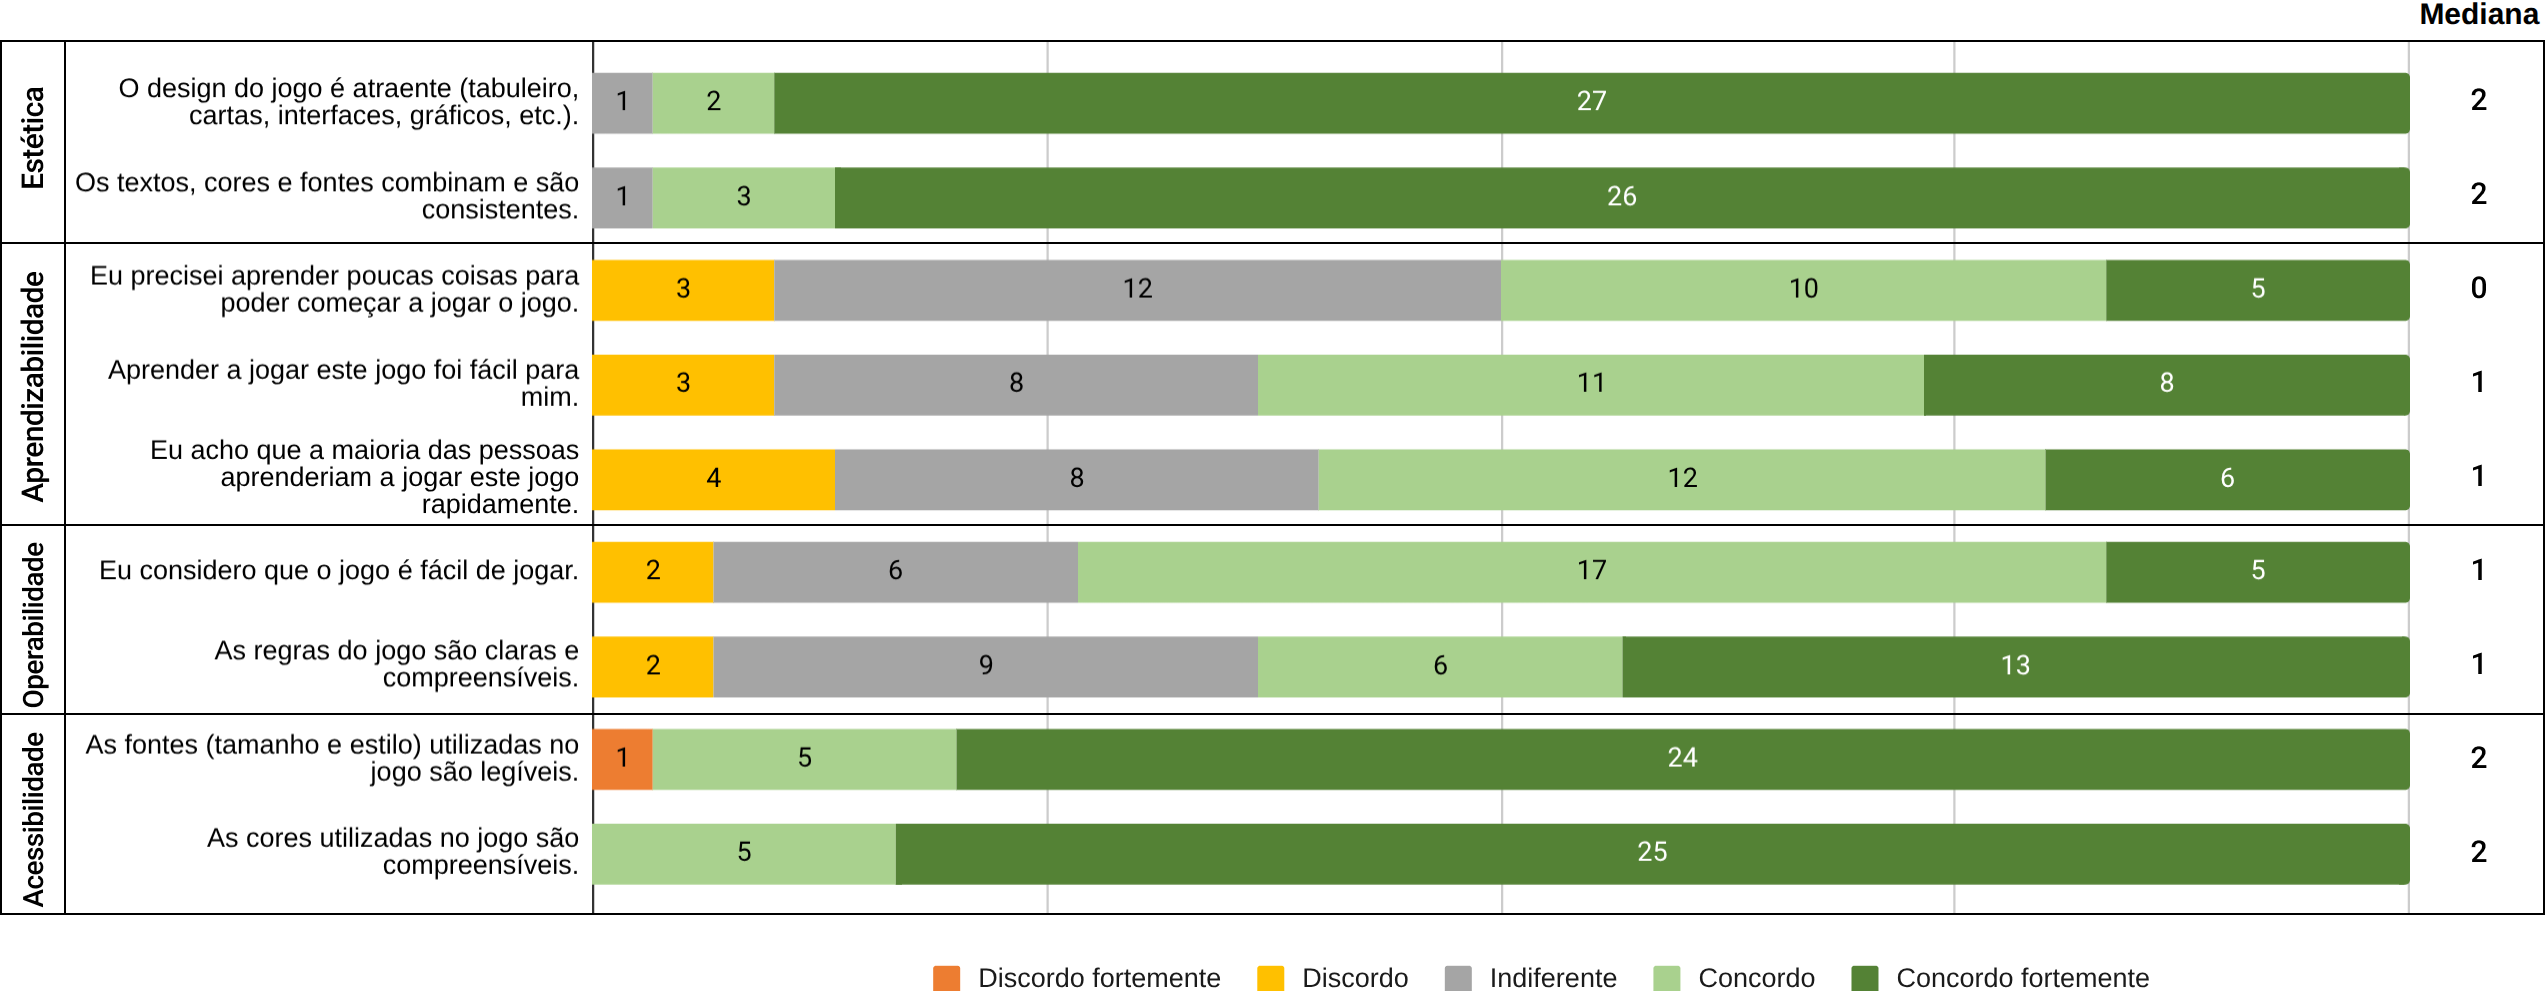
\includegraphics[width=\textwidth]{ufsc-usabilidade}
\end{figure}

Na experiência do jogador, a interação social foi um ponto forte, com mediana de “Concordo fortemente” em todos os itens, destacando a colaboração e engajamento. No entanto, a curva de aprendizado, clareza das regras, facilidade de jogar e o senso de desafio/diversão tiveram medianas ligeiramente menores (“Concordo”) e maior dispersão, sugerindo que o ambiente formal da sala de aula pode ter inibido a imersão lúdica.

\begin{figure}[H]
	\caption{\label{ufsc-xp-jogador} Resultados da avaliação de experiência do jogador com estudantes}
  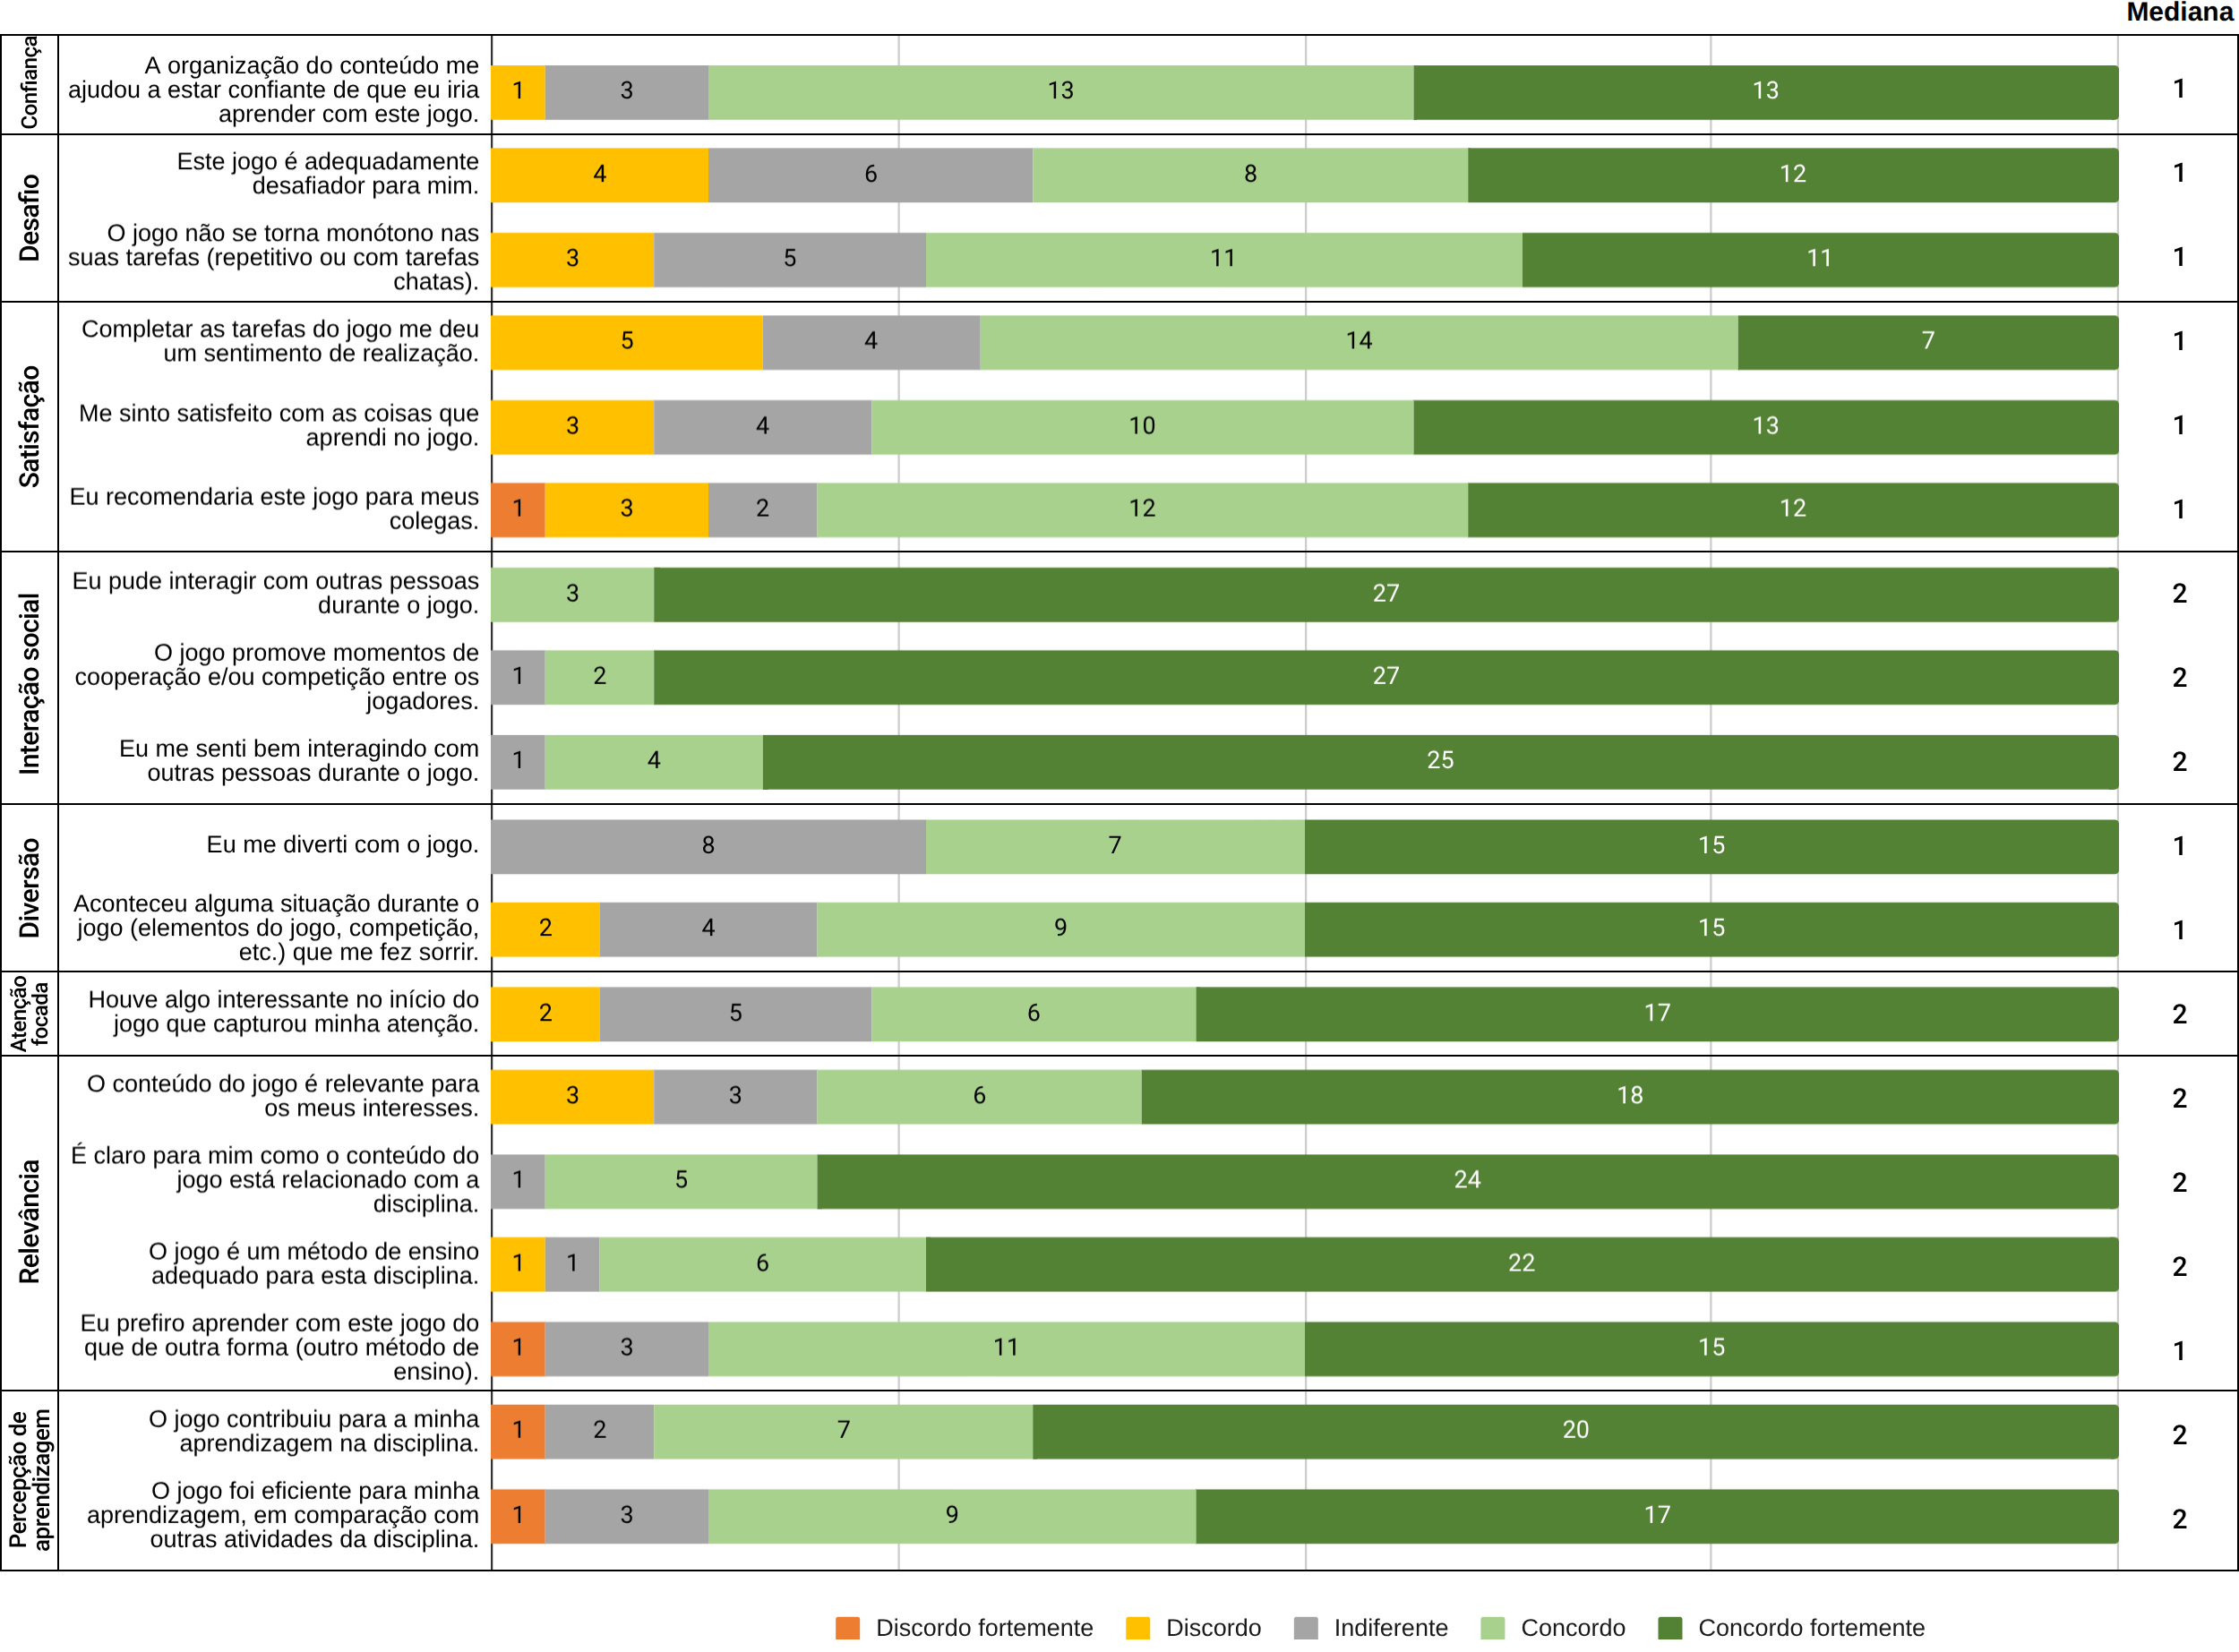
\includegraphics[width=\textwidth]{ufsc-xp-jogador}
\end{figure}

Para os objetivos específicos, a dinâmica foi unanimemente avaliada como bem-sucedida, com mediana de “Concordo fortemente” para todos os itens relacionados à capacidade de despertar a consciência sobre riscos em projetos, promovendo identificação e discussão eficazes.

\begin{figure}[H]
	\caption{\label{ufsc-afirmativas} Resultados da avaliação de afirmativas específicas com estudantes}
  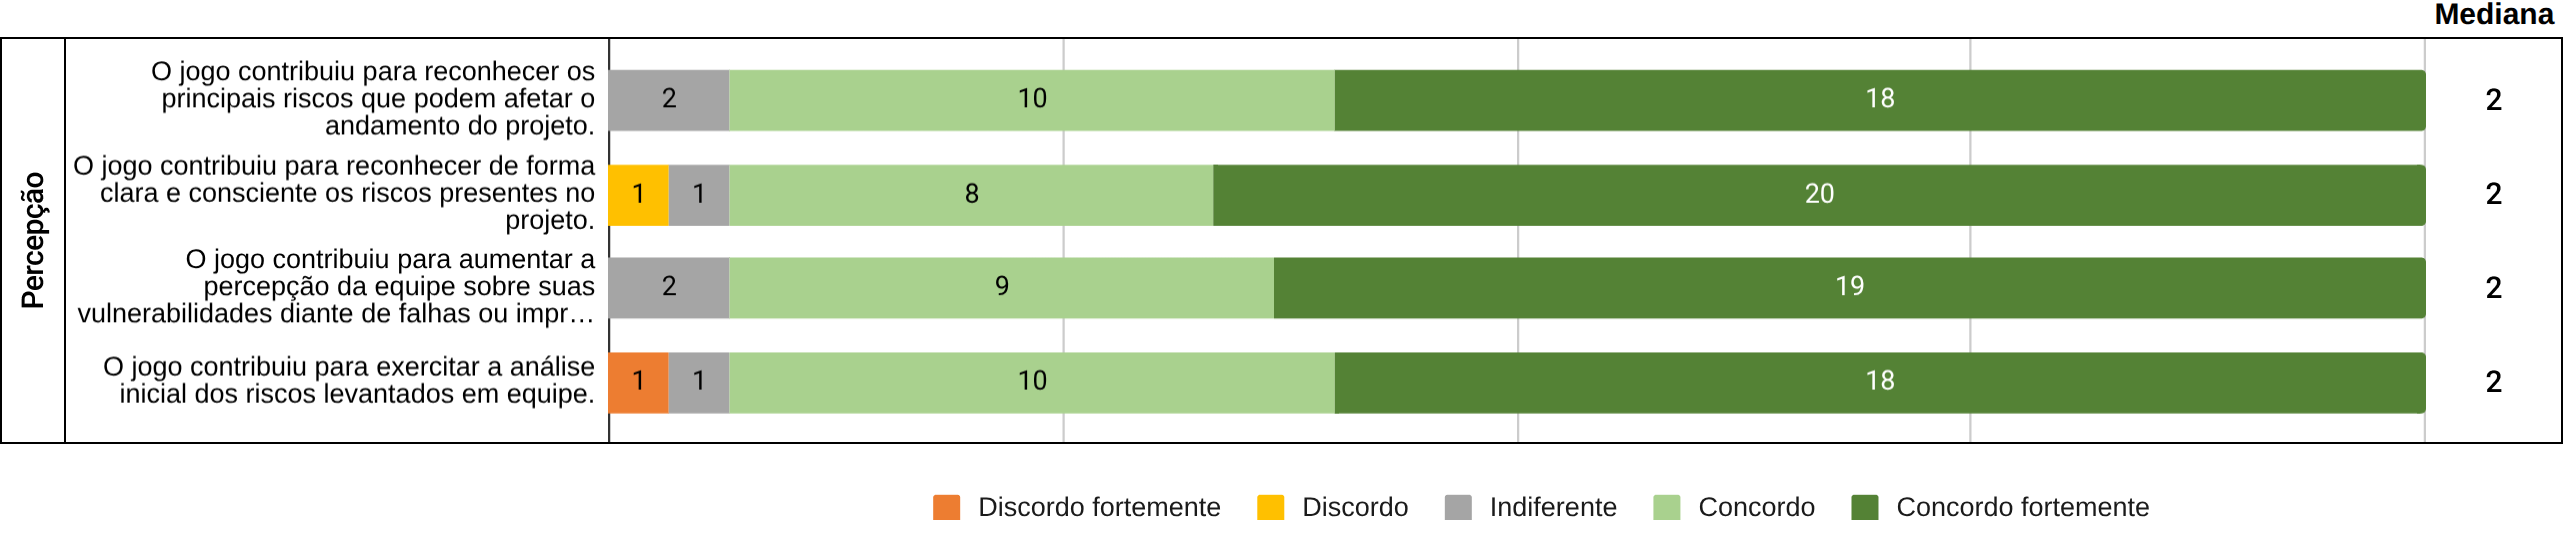
\includegraphics[width=\textwidth]{ufsc-afirmativas}
\end{figure}

O feedback qualitativo elogiou a qualidade e estética do material, a interatividade, a eficácia na identificação e análise de riscos, e a abordagem descontraída. As sugestões de melhoria incluíram revisar o número e a repetitividade das cartas, aprimorar a clareza das regras e o tempo de execução, e oferecer mais detalhes sobre o cenário do projeto fictício ou a estruturação da análise.

\subsection{Resultados com profissionais}
A segunda etapa da avaliação foi realizada com 43 profissionais do mercado de tecnologia do Laboratório Bridge da UFSC. Os participantes, com média de 26 anos, atuam em papéis como Scrum Master, Product Owner, desenvolvedores e designers. A aplicação foi feita de forma online, conduzida pelos próprios Scrum Masters das equipes, utilizando plataformas como Google Meet, Discord e FigJam. As aplicações variaram em número de participantes por equipe (7 a 8), tipo de deck utilizado (básico, completo ou customizado) e tempo médio (60 a 90 minutos).

Em relação à Usabilidade, a dinâmica obteve resultados altamente positivos. Todos os itens relacionados à aparência visual, combinação de cores e fontes, legibilidade e organização do conteúdo obtiveram mediana 2 (“Concordo fortemente”), indicando que a dinâmica é percebida como visual e funcionalmente atrativa. O item “Eu precisei aprender poucas coisas para poder começar a jogar” obteve 88,5\% de concordância, sugerindo que uma clareza adicional nas instruções iniciais pode otimizar a experiência.

\begin{figure}[H]
	\caption{\label{bridge-usabilidade} Resultados da avaliação de usabilidade com profissionais}
  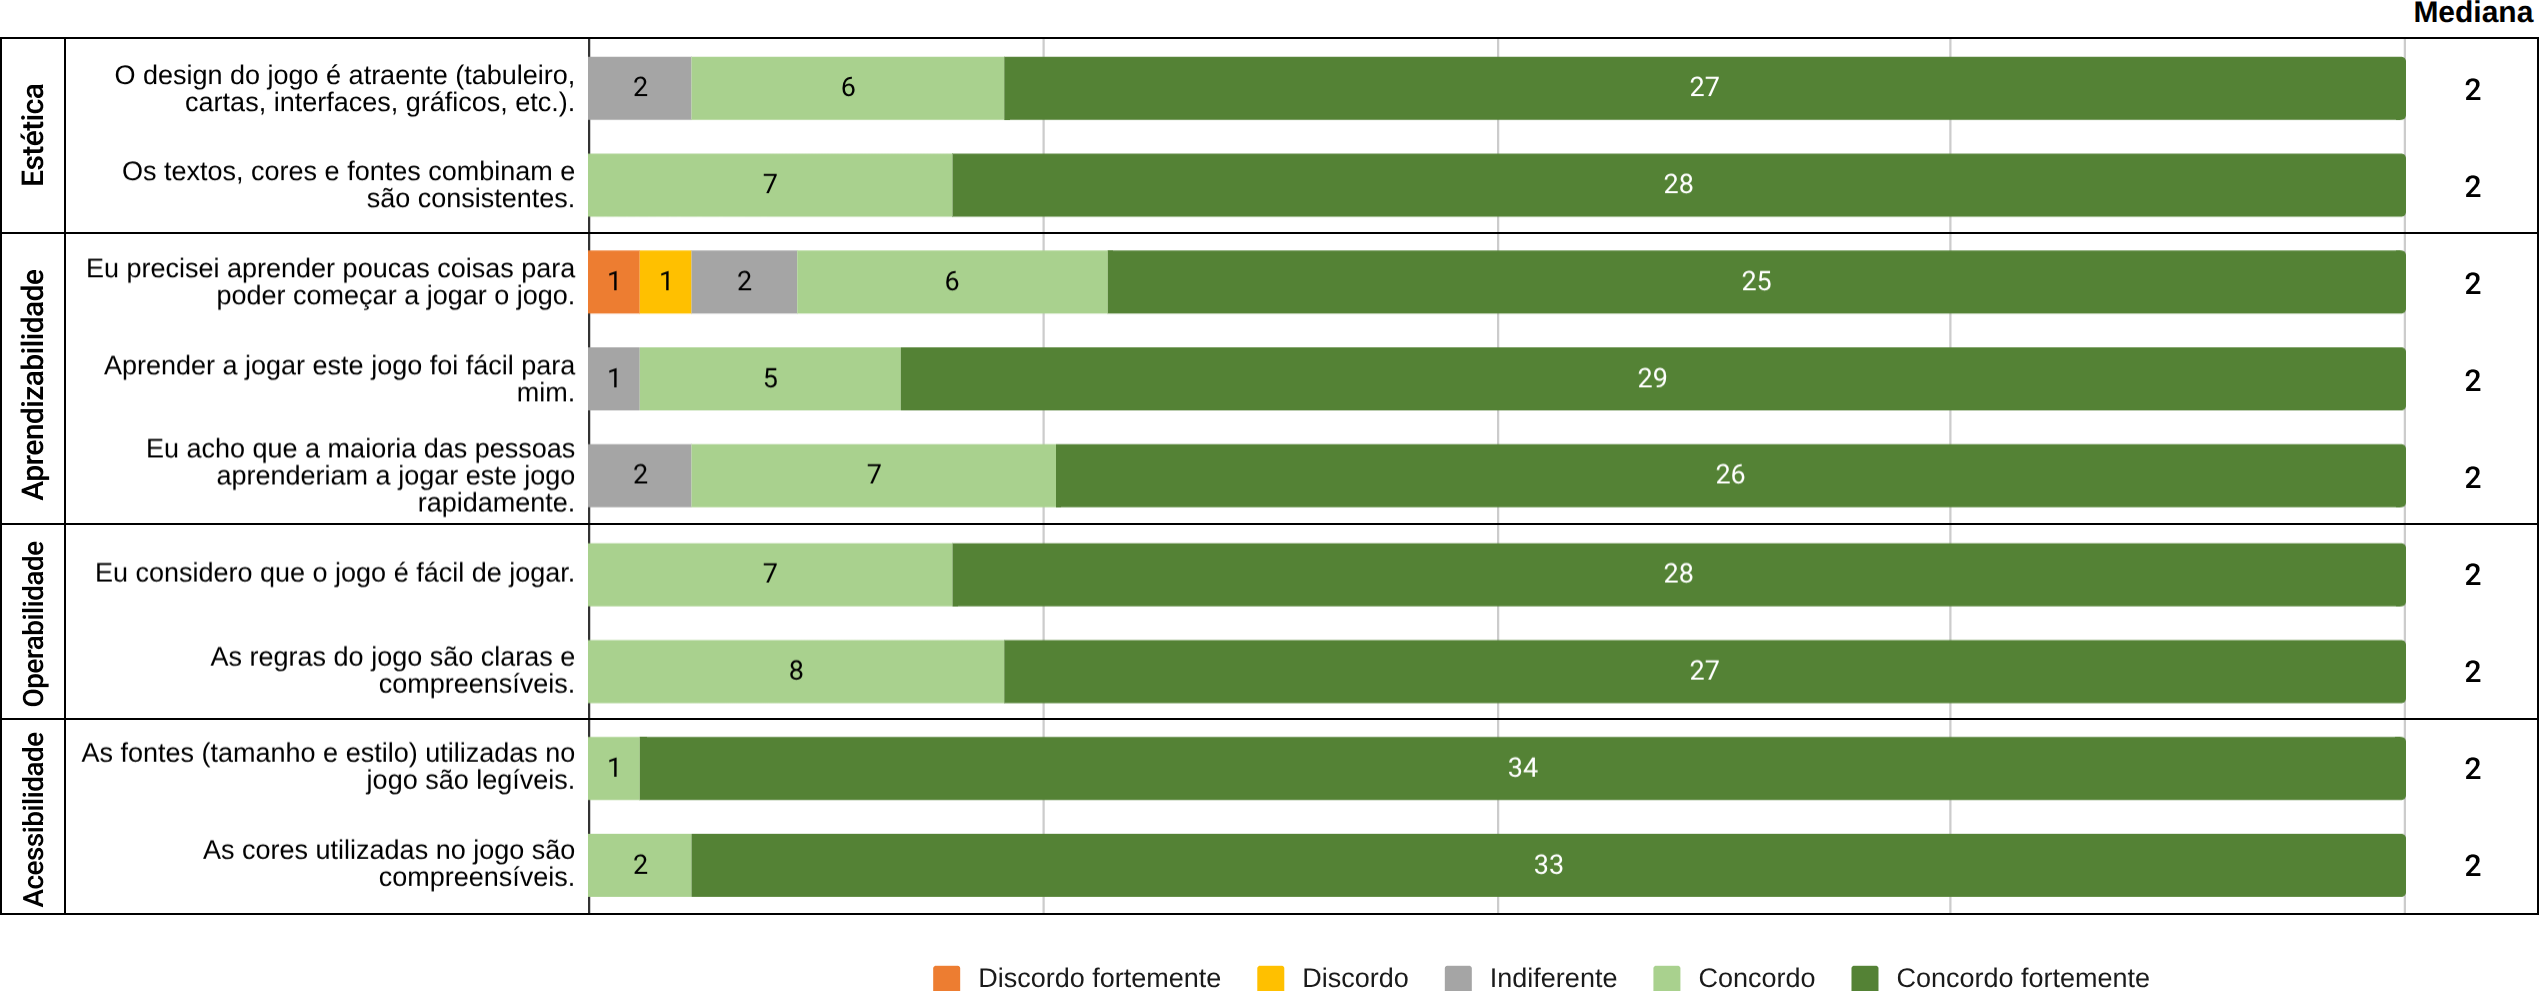
\includegraphics[width=\textwidth]{bridge-usabilidade}
\end{figure}

No critério Experiência do Jogador, a facilidade de aprendizado foi um aspecto crucial, com itens como curva de aprendizado, clareza das regras e facilidade de jogar apresentando mediana 2 (“Concordo fortemente”). Isso demonstra que a dinâmica é intuitiva e acessível, com tempo de adaptação mínimo. Itens relacionados a desafio adequado, tarefas não monótonas e sentimento de realização obtiveram mediana 1 (“Concordo”), indicando oportunidades para aprimoramento no engajamento mais profundo. A dimensão de interação social foi muito bem avaliada, com mediana 2 (“Concordo fortemente”) em todos os seus itens, promovendo um ambiente colaborativo e positivo. Itens de diversão, momentos de alegria, atenção inicial e relevância do conteúdo também obtiveram mediana 2 (“Concordo fortemente”).

\begin{figure}[H]
	\caption{\label{bridge-xp-jogador} Resultados da avaliação de experiência do jogador com profissionais}
  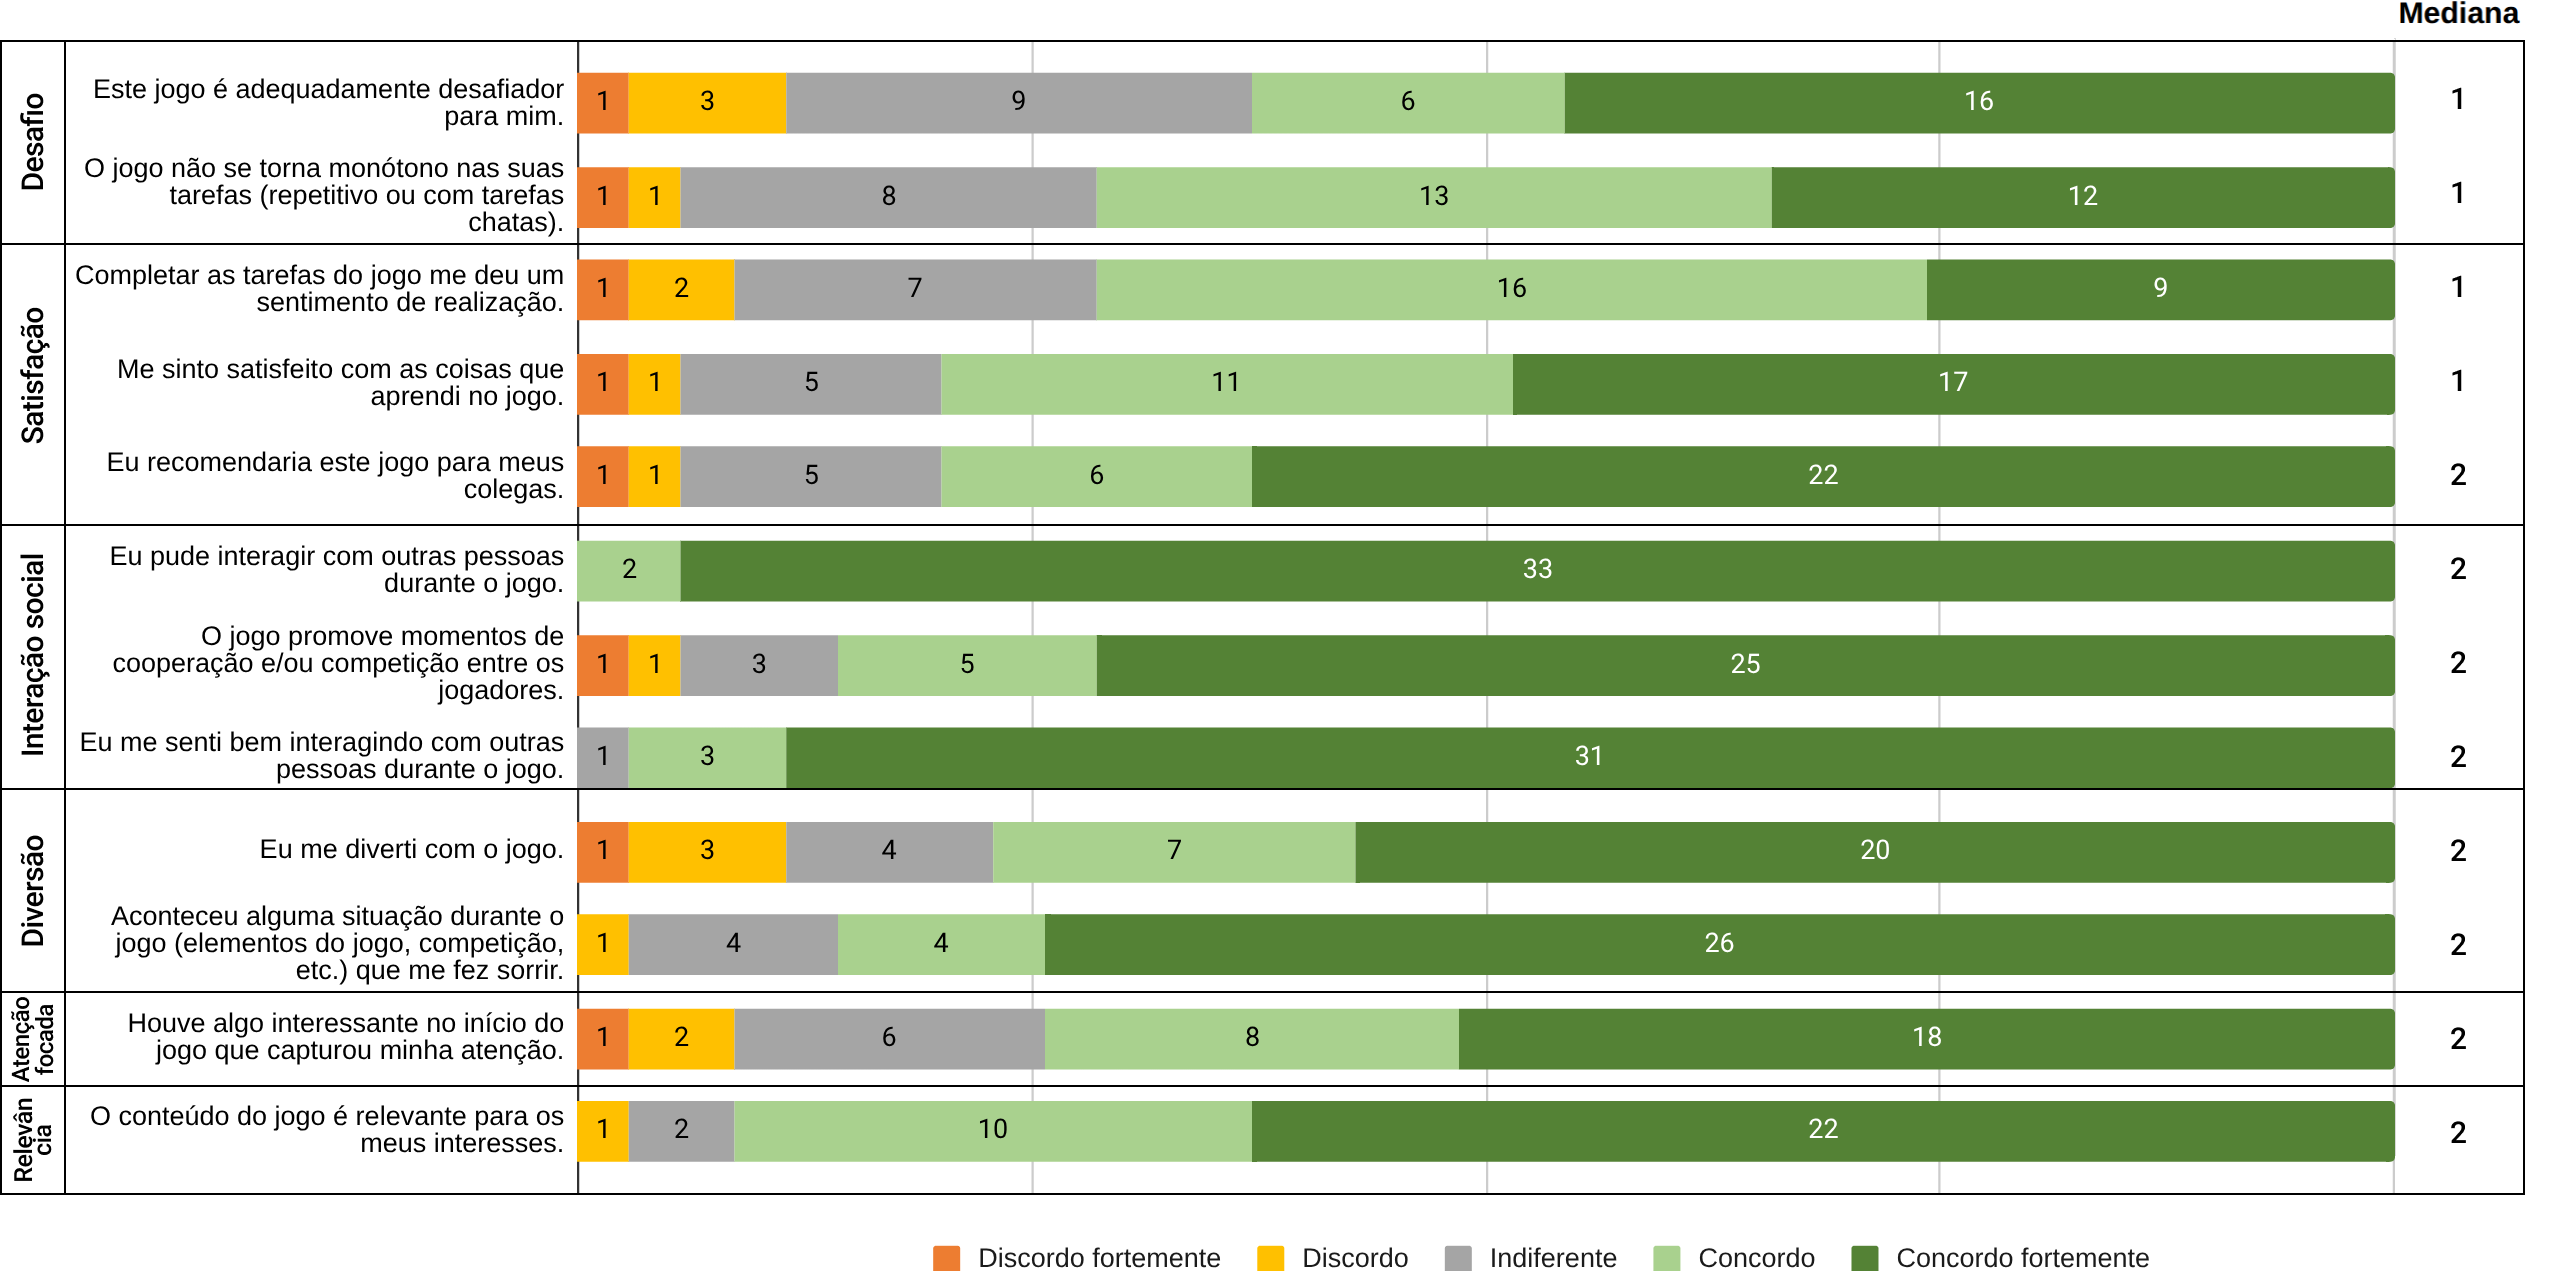
\includegraphics[width=\textwidth]{bridge-xp-jogador}
\end{figure}

Quanto aos objetivos específicos da dinâmica, os itens relacionados à percepção de riscos, vulnerabilidades e análise de riscos obtiveram mediana 2 (“Concordo fortemente”). Isso confirma que a dinâmica cumpre eficazmente sua função de ser útil e diretamente aplicável ao contexto dos projetos dos profissionais.

\begin{figure}[H]
	\caption{\label{bridge-afirmativas} Resultados da avaliação de afirmativas específicas com profissionais}
  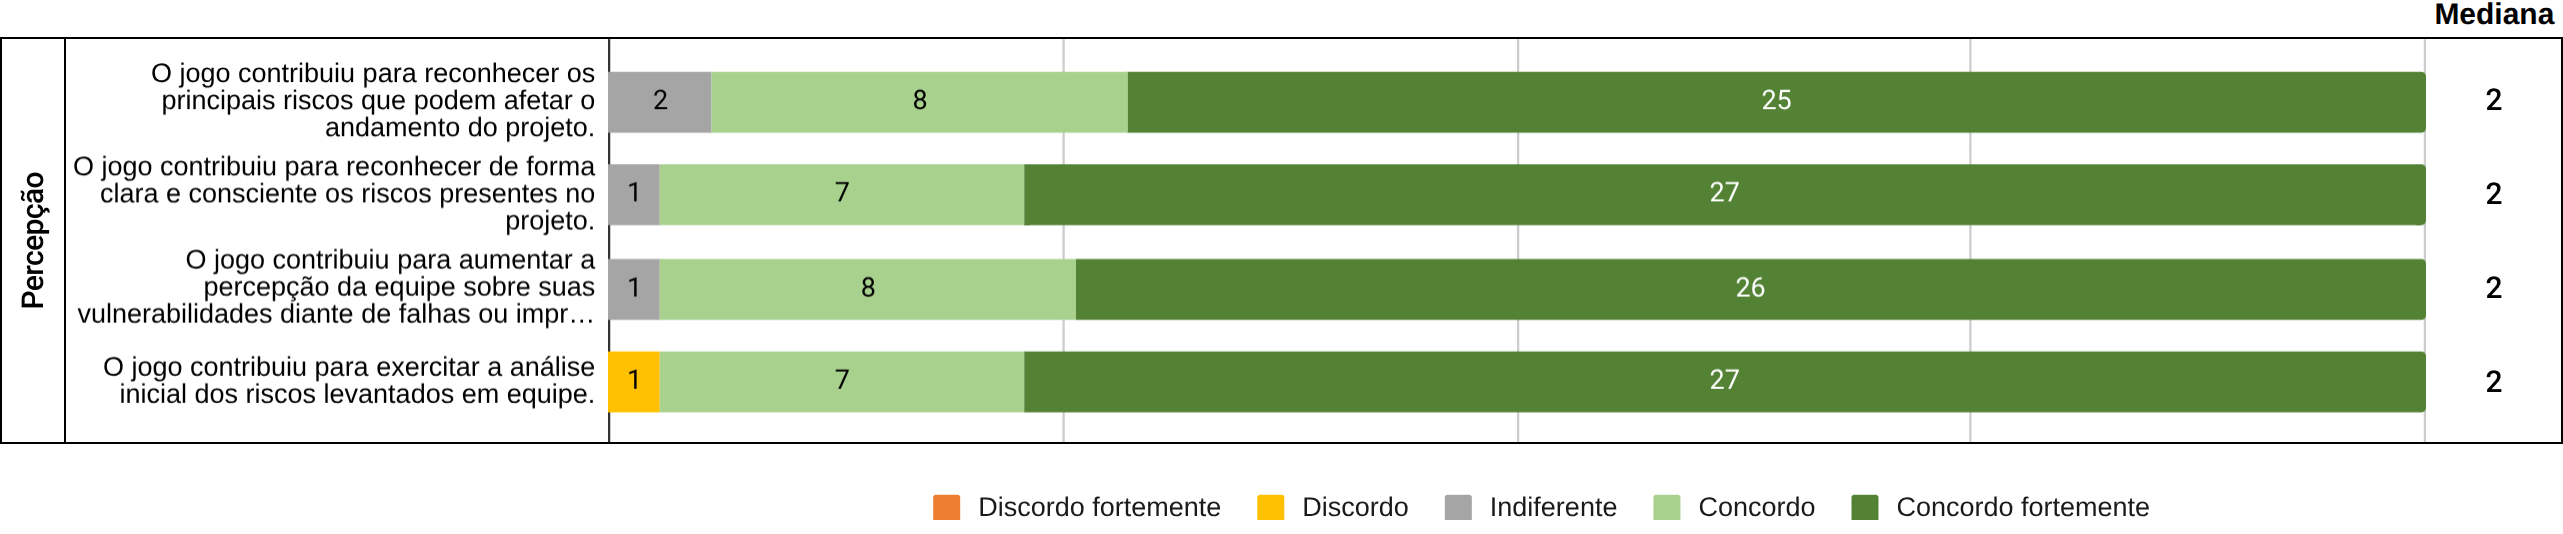
\includegraphics[width=\textwidth]{bridge-afirmativas}
\end{figure}

O feedback qualitativo dos profissionais elogiou a eficácia na identificação e análise de riscos, o formato lúdico e engajador, o estímulo à interação e colaboração, e a organização e clareza do material. As sugestões de aprimoramento incluíram a duração ideal (cerca de 1 hora para o deck completo), a repetitividade e sobreposição de cartas, clareza e formatação das perguntas, melhorias na ferramenta digital (como um aplicativo próprio) e a necessidade de aprofundamento pós-dinâmica (módulo para planos de ação).

\subsection{Discussão}
%A análise dos resultados demonstra que a dinâmica “Tarot dos Riscos” atendeu aos objetivos propostos e tem potencial para ser incorporada como uma ferramenta prática no cotidiano de equipes ágeis. O formato gamificado contribuiu para o engajamento dos participantes, enquanto as perguntas das cartas fomentaram discussões relevantes sobre riscos. A combinação de aspectos lúdicos com conteúdo técnico mostrou-se eficaz para abordar um tema que tradicionalmente recebe pouca atenção.

Este capítulo apresentou a avaliação da dinâmica, comparando os resultados quantitativos e as percepções qualitativas de estudantes de graduação e profissionais atuantes no mercado. Apesar das diferenças entre os públicos e ambientes, a dinâmica demonstrou consistentemente pontos fortes em diversas dimensões. O design visual e a clareza da apresentação foram universalmente bem avaliados, contribuindo positivamente para a experiência inicial. A interação social foi um ponto de excelência, com todos os itens sociais obtendo mediana 2 (“Concordo fortemente”) em ambos os grupos, evidenciando a capacidade da dinâmica em promover colaboração e engajamento. Adicionalmente, os objetivos específicos da dinâmica foram consistentemente bem avaliados, atingindo mediana 2 (“Concordo fortemente”), confirmando que a ferramenta auxilia na identificação e discussão de riscos de forma eficaz e didática.

A comparação entre os grupos revelou discrepâncias importantes para o aprimoramento da dinâmica. A facilidade de aprendizado foi significativamente menor para estudantes (mediana 0 - “Indiferente” para “Eu precisei aprender poucas coisas para começar a jogar o jogo”) em contraste com os profissionais (mediana 2 - “Concordo fortemente”). Isso sugere que o tempo limitado em sala de aula ou a menor familiaridade com o formato podem exigir um processo de onboarding mais robusto para ambientes acadêmicos. Quanto ao engajamento emocional e diversão, os profissionais avaliaram com medianas mais altas (mediana 2 - “Concordo fortemente” para “Me diverti com o jogo” e “Aconteceu algo no jogo que me fez sorrir”) do que os estudantes (mediana 1 - “Concordo”). Essa diferença indica que o aspecto lúdico e a sensação de conquista foram não puderam ser observado no contexto acadêmico, apontando a necessidade de se criar um clima mais descontraído para otimizar o engajamento lúdico nesses contextos. Em síntese, embora a dinâmica demonstre um desempenho visual e pedagógico elevado, ajustes no onboarding e na ambientação são necessários para maximizar seu potencial em diferentes contextos.

\subsubsection{Ameaças à validade}

A condução deste estudo empírico está sujeita a diversas ameaças à validade que podem limitar a generalização e a confiança nos resultados. Em relação à validade de construto, as ameaças incluem a subjetividade das percepções dos participantes, a interpretação das perguntas do questionário, a adaptação do instrumento MEEGA+, que pode comprometer suas propriedades psicométricas originais, e o efeito Hawthorne, onde a participação no estudo pode influenciar as respostas. As mitigações envolvem a triangulação de dados (qualitativos e quantitativos), clareza na redação das perguntas e a garantia de anonimato.

Para a validade interna, as diferenças entre os grupos de aplicação (estudantes vs. profissionais, presencial vs. online), o envolvimento e potencial viés da pesquisadora, a maturação e eventos históricos externos podem influenciar a relação de causa e efeito. A mitigação incluiu a análise separada dos grupos e a aplicação por terceiros em parte dos casos.

A validade externa é ameaçada pela estratégia de seleção da amostra (conveniência e vínculos pessoais), o contexto específico de aplicação (sala de aula e laboratório) e a modalidade de aplicação (remota via FigJam para a maioria dos profissionais). A mitigação busca descrever o perfil dos participantes e o contexto para permitir a avaliação de similaridade em futuras replicações.

Por fim, a validade de conclusão é afetada pelo tamanho moderado da amostra e pela variabilidade dentro dos grupos. A análise baseada em medianas e frequências percentuais, complementada por dados qualitativos, foi usada para mitigar essas limitações.

\section{Conclusão}

Este trabalho focou no desenvolvimento e avaliação de uma dinâmica gamificada para auxiliar na análise e identificação de riscos em equipes ágeis de desenvolvimento de software. A pesquisa foi embasada em sólida fundamentação teórica e um mapeamento sistemático da literatura, que revelou a necessidade de ferramentas mais interativas para a gestão de riscos.

A avaliação, realizada com estudantes e profissionais, demonstrou que a dinâmica é promissora e eficaz, engajando os participantes e promovendo a colaboração na identificação e análise de riscos. O design visual e a interação social foram consistentemente bem avaliados, e a dinâmica cumpriu seus objetivos pedagógicos e práticos. Embora a facilidade de aprendizado e o engajamento lúdico tenham sido mais acentuados entre profissionais, a dinâmica mostrou um desempenho visual e pedagógico elevado, validando sua concepção.

\bibliographystyle{sbc}
\bibliography{artigo}

\end{document}
